\documentclass{standalone}
\usepackage{tikz}

\begin{document}
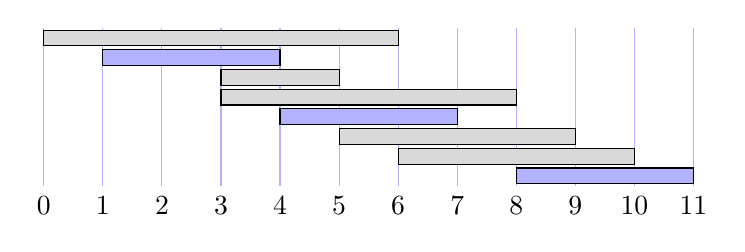
\begin{tikzpicture}[yscale = .25, xscale =.75, fill = black!20, text = black]
  \foreach \i in {0,...,11}
  {
  \draw [thin, blue!30] (\i, -8) -- (\i, 0);
  \node [fill = none] at (\i, -9) {\i};
}

\draw [fill = gray!30] (0, -0.1) rectangle ( 6, -0.9) ;
\draw [fill = blue!30] (1, -1.1) rectangle ( 4, -1.9) ;
\draw [fill = gray!30] (3, -2.1) rectangle ( 5, -2.9) ;
\draw [fill = gray!30] (3, -3.1) rectangle ( 8, -3.9) ;
\draw [fill = blue!30] (4, -4.1) rectangle ( 7, -4.9) ;
\draw [fill = gray!30] (5, -5.1) rectangle ( 9, -5.9) ;
\draw [fill = gray!30] (6, -6.1) rectangle (10, -6.9) ;
\draw [fill = blue!30] (8, -7.1) rectangle (11, -7.9) ;
\end{tikzpicture}
\end{document}

